% The three figures belonging to §6. Held in their own file so main.tex and review_s6.tex
% share one copy and the export cannot drift from the manuscript.
\begin{figure}[t]
  \centering
  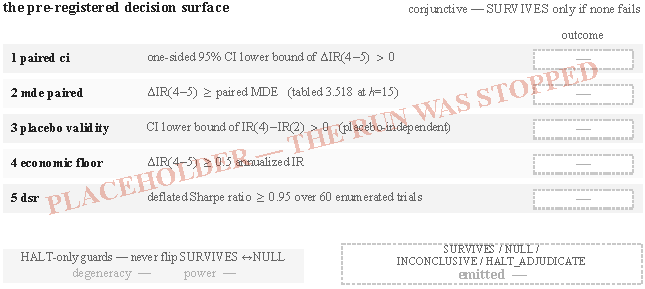
\includegraphics[width=\textwidth]{figures/fig8_verdict.pdf}
  \caption{\textbf{The decision surface, fixed before any result existed.} Five clauses, evaluated
  conjunctively: the primary outcome is SURVIVES only if none fails, and NULL otherwise. Two
  guards sit outside the clauses and are HALT-only --- they can refuse to report an outcome their
  own inputs cannot support, and can never flip SURVIVES to NULL or back. The rule strings shown
  are transcribed into this figure's source rather than loaded from a manifest, and are therefore a
  restatement; the persisted strings are the authority. \PH{no values} --- every outcome
  cell is empty because the run has not been executed; each is filled from a single named field of
  that manifest.}
  \label{fig:verdict}
\end{figure}
\clearpage
\begin{figure}[t]
  \centering
  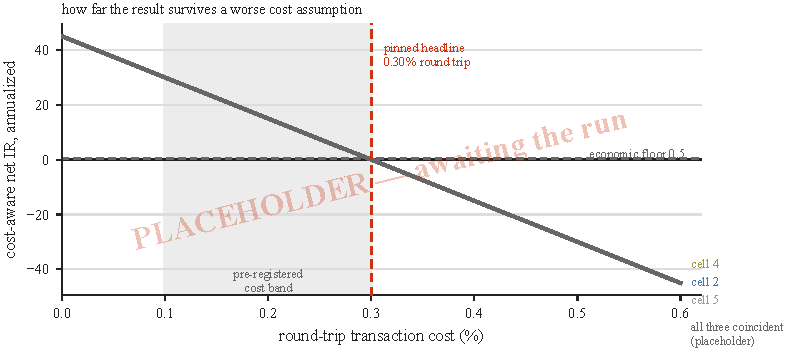
\includegraphics[width=\textwidth]{figures/fig9_cost_stress.pdf}
  \caption{\textbf{The specified cost-stress apparatus, with no curve.} Cost-aware net information
  ratio against the round-trip transaction cost was to be drawn here for the microstructure arm,
  the OHLCV-only arm and the placebo; the headline is pinned at $0.30\%$, the pessimistic end of
  the pre-registered $0.1$--$0.3\%$ band. \PH{no curve drawn} --- the ablation this panel was
  specified for never ran, so the axes, the pinned rate, the band and the economic floor are real
  and no cell is drawn. An earlier draft carried a placeholder line whose zero crossing fell
  \emph{exactly} on the pinned $0.30\%$ rule, the most quotable point on the axis; cropped away
  from this caption it read as a break-even of $0.30\%$, against a measured $0.0023$--$0.0208\%$.
  The one break-even we have measured is drawn instead, in red at the left margin, with its
  cell-1-only scope written into the image rather than left to the caption.}
  \label{fig:cost}
\end{figure}
\clearpage
\begin{figure}[t]
  \centering
  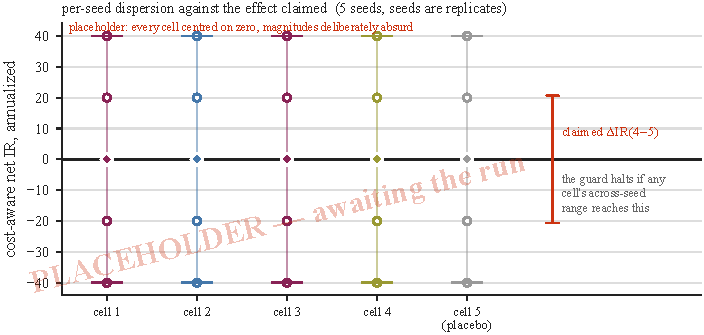
\includegraphics[width=\textwidth]{figures/fig10_seed_stability.pdf}
  \caption{\textbf{Seed dispersion against the effect being claimed.} Each cell's five seeds are
  replicates of one configuration, not five configurations; open circles are seeds, the diamond is
  the seed mean, and the bars mark the across-seed range. The comparison that matters is the one
  drawn on the right: if any cell's across-seed range reaches the size of the effect being claimed,
  the power guard halts and the verdict is reported as adjudication-required rather than as an
  outcome.
  \PH{every cell centred on zero, magnitudes $\sim\pm40$} --- no cell is favoured and the claimed
  effect is drawn symmetric about zero, so the panel shows the comparison's geometry and no
  result.}
  \label{fig:seeds}
\end{figure}
\clearpage

